\documentclass[12pt, twoside]{book}
%\documentclass[12pt, oneside]{book}  % jednostranna tlac
\usepackage[a4paper,top=2.5cm,bottom=2.5cm,left=3.5cm,right=2cm]{geometry}
\usepackage[utf8]{inputenc}
\usepackage[T1]{fontenc}
\usepackage{graphicx}
\usepackage{url}
\usepackage[hidelinks,breaklinks]{hyperref}
\usepackage{float}
%\usepackage[slovak]{babel} % vypnite pre prace v anglictine
\linespread{1.25} % hodnota 1.25 by mala zodpovedat 1.5 riadkovaniu

% CUSTOM THINGS
\newtheorem{theorem}{Definition}[section]
\newtheorem{corollary}{Corollary}[theorem]
\newtheorem{lemma}[theorem]{Lemma}
\usepackage{amsmath}

% -------------------
% --- Definicia zakladnych pojmov
% --- Vyplnte podla vasho zadania
% -------------------
\def\mfrok{2021}
\def\mfnazov{Trusted Types integration into open source frameworks and libraries}
\def\mftyp{Masters Thesis}
\def\mfautor{Emanuel Tesař, Bc.}
\def\mfskolitel{RNDr. Peter Borovanský, PhD.}

%ak mate konzultanta, odkomentujte aj jeho meno na titulnom liste, TODO: maybe add koto
% \def\mfkonzultant{tit. Meno Priezvisko, tit. }  

\def\mfmiesto{Bratislava, \mfrok}

% bioinformatici odkomentujú riadok s dvoma odbormi a iný program
\def\mfodbor{Computer Science}
%\def\mfodbor{Computer Science and Biology} 
\def\program{Computer Science}
%\def\program{ Bioinformatics }

% Ak je školiteľ z FMFI, uvádzate katedru školiteľa, zrejme by mala byť aj na zadaní z AIS2
% Ak máte externého školiteľa, uvádzajte Katedru informatiky 
\def\mfpracovisko{ FMFI.KAI - Department of Applied Informatics }

\begin{document}
\frontmatter


% -------------------
% --- Obalka ------
% -------------------
\thispagestyle{empty}

\begin{center}
  \sc\large
  Comenius University in Bratislava\\
  Faculty of Mathematics, Physics and Informatics

  \vfill

  {\LARGE\mfnazov}\\
  \mftyp
\end{center}

\vfill

{\sc\large
  \noindent \mfrok\\
  \mfautor
}

\cleardoublepage
% --- koniec obalky ----

% -------------------
% --- Titulný list
% -------------------

\thispagestyle{empty}
\noindent

\begin{center}
  \sc
  \large
  Comenius University in Bratislava\\
  Faculty of Mathematics, Physics and Informatics

  \vfill

  {\LARGE\mfnazov}\\
  \mftyp
\end{center}

\vfill

\noindent
\begin{tabular}{ll}
  Study Programme: & \program      \\
  Field of Study:  & \mfodbor      \\
  Department:      & \mfpracovisko \\
  Supervisor:      & \mfskolitel   \\
  % Consultant: & \mfkonzultant \\
\end{tabular}

\vfill


\noindent \mfmiesto\\
\mfautor

\cleardoublepage
% --- Koniec titulnej strany


% -------------------
% --- Zadanie z AIS
% -------------------
% v tlačenej verzii s podpismi zainteresovaných osôb.
% v elektronickej verzii sa zverejňuje zadanie bez podpisov
% v pracach v naglictine anglicke aj slovenske zadanie

\newpage
\thispagestyle{empty}
% TODO: updatni zadania z AISu ked sa praca schvali
% \hspace{-2cm}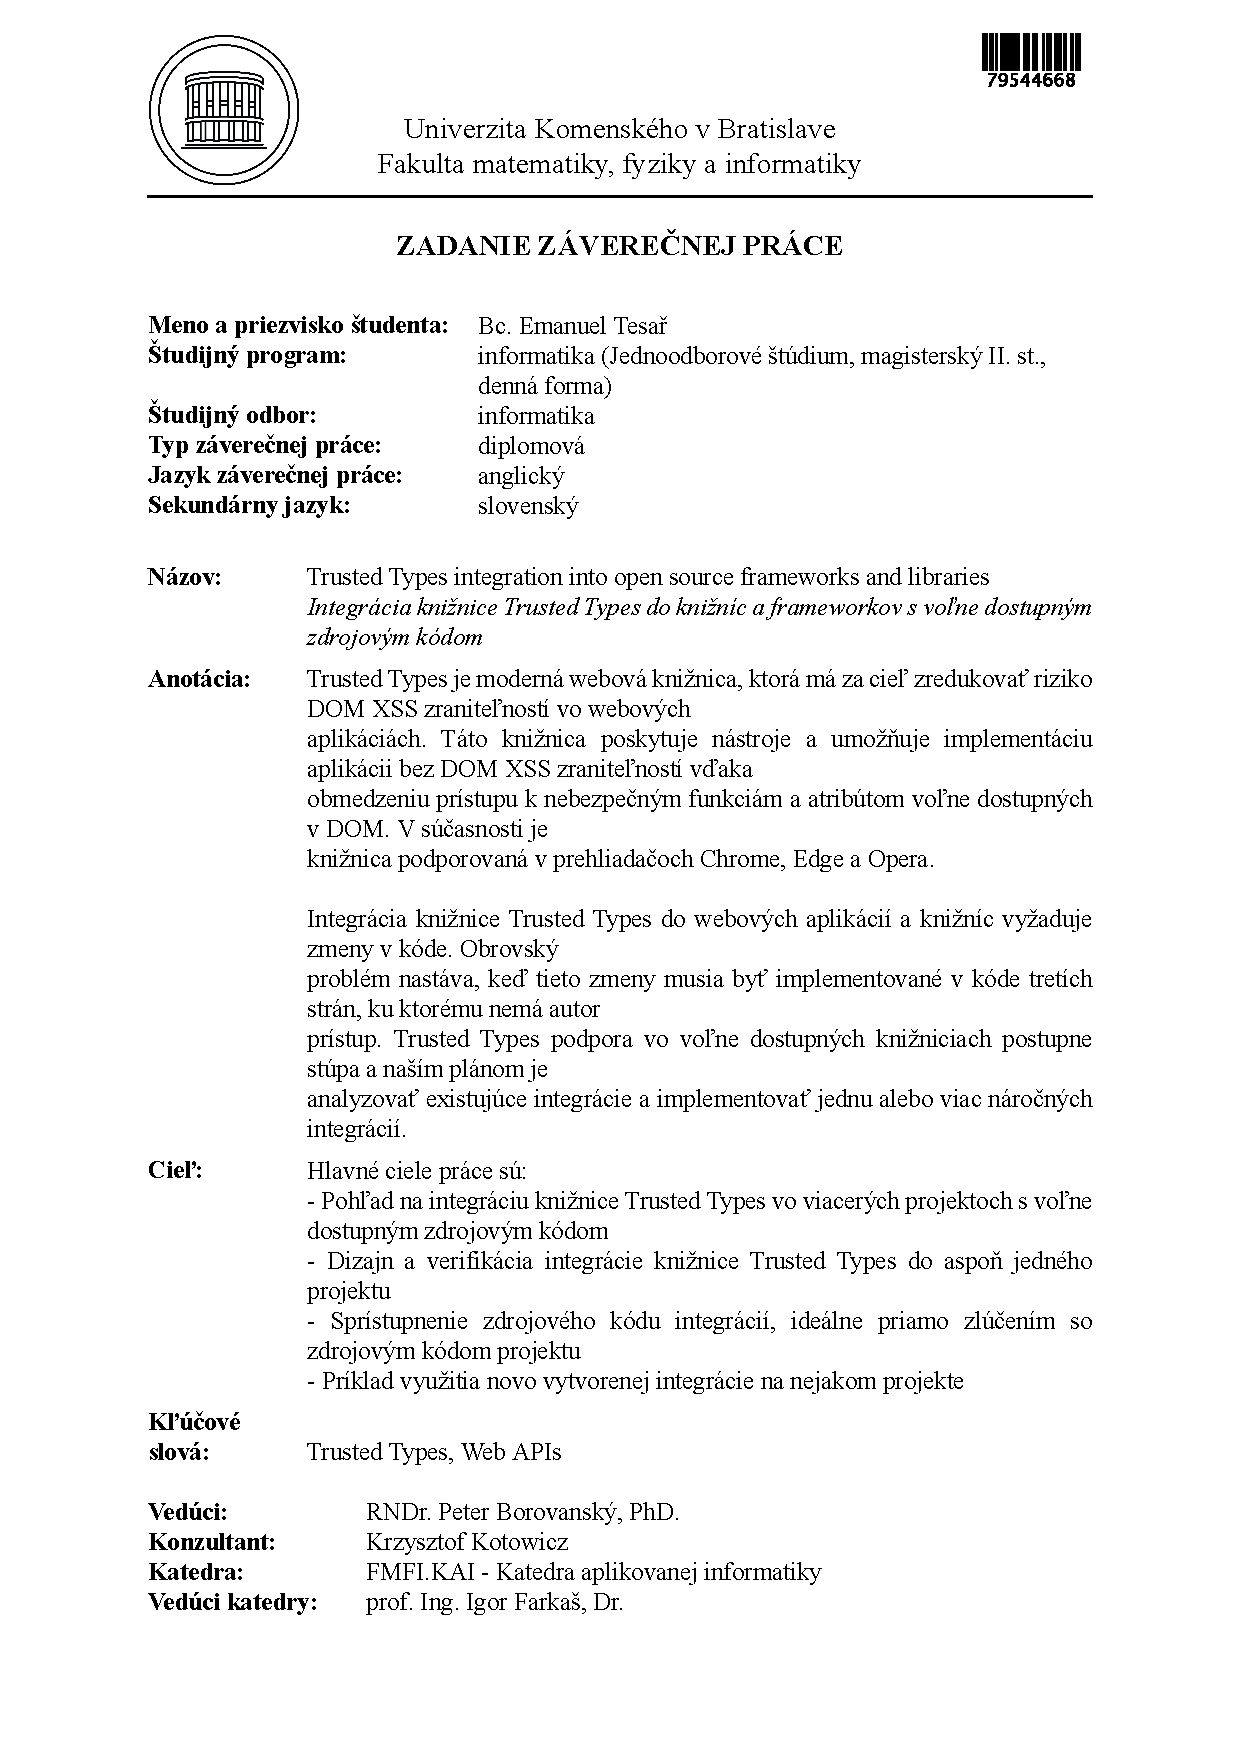
\includegraphics[width=1.1\textwidth]{images/zadanie}

% \hspace{-2cm}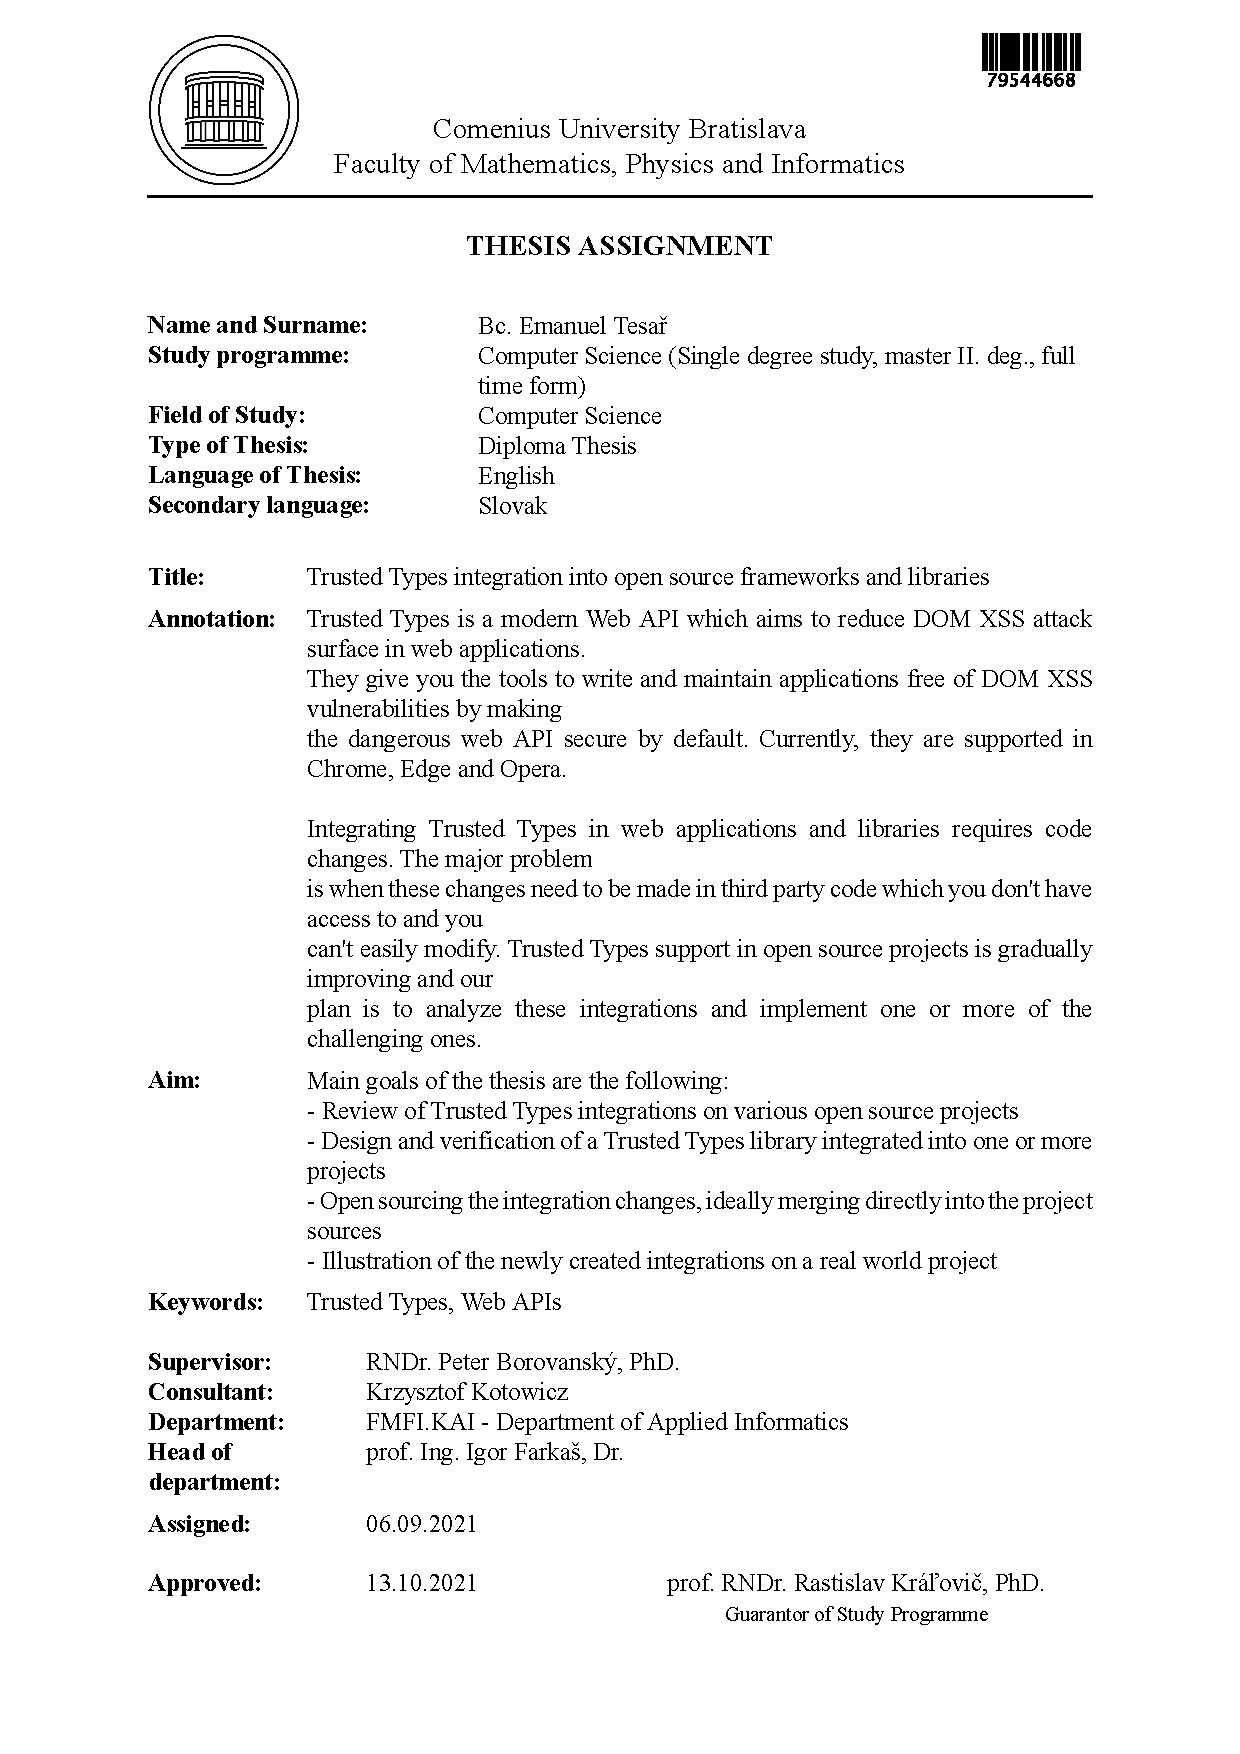
\includegraphics[width=1.1\textwidth]{images/zadanie-en}

% --- Koniec zadania

\frontmatter

% -------------------
%   Poďakovanie - nepovinné
% -------------------
\setcounter{page}{3}
\newpage
~

\vfill
% TODO: acknowledgments
{\bf Acknowledgments:}

% --- Koniec poďakovania

% -------------------
%   Abstrakt - Slovensky
% -------------------
\newpage
\section*{Abstrakt}

% TODO: fill SK abstract

% TODO: fill in most suitable keywords when the thesis is done
\paragraph*{Kľúčové slová: Trusted Types, Web APIs}
% --- Koniec Abstrakt - Slovensky


% -------------------
% --- Abstrakt - Anglicky 
% -------------------
\newpage
\section*{Abstract}

% TODO: fill EN abstract

% TODO: fill in most suitable keywords when the thesis is done
\paragraph*{Keywords: Trusted Types, Web APIs}

% --- Koniec Abstrakt - Anglicky

% -------------------
% --- Predhovor - v informatike sa zvacsa nepouziva
% -------------------
%\newpage 
%\thispagestyle{empty}
%
%\huge{Predhovor}
%\normalsize
%\newline
%Predhovor je všeobecná informácia o práci, obsahuje hlavnú charakteristiku práce 
%a okolnosti jej vzniku. Autor zdôvodní výber témy, stručne informuje o cieľoch 
%a význame práce, spomenie domáci a zahraničný kontext, komu je práca určená, 
%použité metódy, stav poznania; autor stručne charakterizuje svoj prístup a svoje 
%hľadisko. 
%
% --- Koniec Predhovor


% -------------------
% --- Obsah
% -------------------

\newpage

\tableofcontents

% ---  Koniec Obsahu

% -------------------
% --- Zoznamy tabuliek, obrázkov - nepovinne
% -------------------

\newpage

\listoffigures
\listoftables

% ---  Koniec Zoznamov

\mainmatter


% \input uvod.tex 

% \input dnaSequencing.tex

% \input sequenceAlignment.tex
%\input latex.tex

%\input lorem.tex

%\input zaver.tex

% -------------------
% --- Bibliografia
% -------------------


\newpage

\backmatter

\thispagestyle{empty}
\nocite{*}
\clearpage

\bibliographystyle{plain}
\bibliography{literatura}

%Prípadne môžete napísať literatúru priamo tu
%\begin{thebibliography}{5}

%\bibitem{br1} MOLINA H. G. - ULLMAN J. D. - WIDOM J., 2002, Database Systems, Upper Saddle River : Prentice-Hall, 2002, 1119 s., Pearson International edition, 0-13-098043-9

%\bibitem{br2} MOLINA H. G. - ULLMAN J. D. - WIDOM J., 2000 , Databasse System implementation, New Jersey : Prentice-Hall, 2000, 653s., ???

%\bibitem{br3} ULLMAN J. D. - WIDOM J., 1997, A First Course in Database Systems, New Jersey : Prentice-Hall, 1997, 470s., 

%\bibitem{br4} PREFUSE, 2007, The Prefuse visualization toolkit,  [online] Dostupné na internete: <http://prefuse.org/>

%\bibitem{br5} PREFUSE Forum, Sourceforge - Prefuse Forum,  [online] Dostupné na internete: <http://sourceforge.net/projects/prefuse/>

%\end{thebibliography}

%---koniec Referencii

% -------------------
%--- Prilohy---
% -------------------

%Nepovinná časť prílohy obsahuje materiály, ktoré neboli zaradené priamo  do textu. Každá príloha sa začína na novej strane.
%Zoznam príloh je súčasťou obsahu.
%
%\input appendixA.tex

%\input appendixB.tex

\end{document}
